\documentclass[12pt]{article}
\usepackage[a4paper, margin=.30in]{geometry}
\usepackage{graphicx ,
            wrapfig,
            xcolor, 
            enumerate,
            amsmath,fontenc,mathrsfs
            }

\newcommand\headerMe[2]{\noindent{}#1\hfill#2}
\renewcommand{\thesection}{\Roman{section}}

\title{Leçon N 6 :Moment d'un couple de forces –Moment d'un couple de torsion }
\author{Zakaria HAOUZAN}
\date{\today}

\begin{document}
% headers --------------
\headerMe{Matière : Physique-Chimie}{Professeur : Zakaria HAOUZAN}\\
\headerMe{Unité : La Mécanique}{Établissement : Lycée SKHOR qualifiant}\\
\headerMe{Niveau : TCS}{Heure : 2H}\\

% ------Content ________
\begin{center}
    \Large{Leçon $N^{\circ}6$: \color{red} Moment d'un couple de forces –Moment d'un couple de torsion }
\end{center}

%\begin{wrapfigure}{r}{0.2\textwidth}
%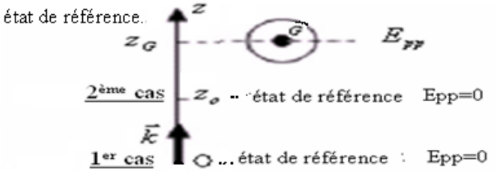
\includegraphics[width=0.2\textwidth]{./img/img00.png}
%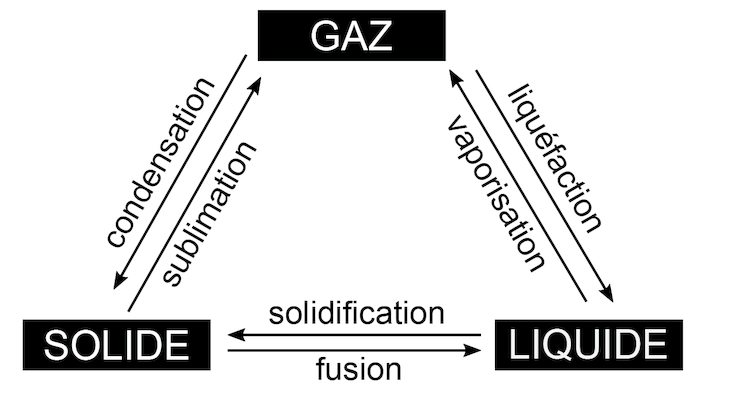
\includegraphics[width=0.2\textwidth]{./img/img01.jpg}
%\end{wrapfigure}


\section{Moment d'un couple de forces: }

\subsection{Notion de couple de forces:}

Un couple de force est un ensemble de deux forces parallèles ,de même intensité, et de sens contraires. ( le couple
de force tend à faire tourner le corps auquel il s'applique).

\textbf{Exemple : }
\begin{itemize}

	\item Pour ouvrir un robinet on applique un couple de force.
\item Pour faire tourner le volant de la voiture
on applique un couple force
\end{itemize}


\subsection{Détermination du moment d'un couple de force: }

\begin{wrapfigure}{r}{0.2\textwidth}
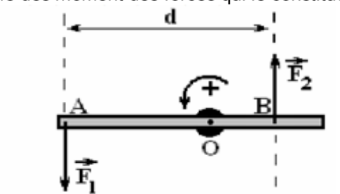
\includegraphics[width=0.2\textwidth]{./img/rotation.png}
\end{wrapfigure}

Le moment du couple de force est la somme des moment des forces qui le constitue :

$\mathscr{M}_{\Delta}(C) = \mathscr{M}_{\Delta}(\vec{F}_1) + \mathscr{M}_{\Delta}(\vec{F}_2) = F_1.d_1 + F_2.d_2$

avec $F_1 = F_2 = F$ et $d_1 + d_2 = d$ d est la distance séparant les deux droites d action.
$$
  \mathscr{M}_\Delta = F.d
$$

Puisque tout couple de force possède un sens qui correspond au sens de rotation qu'il tend à produire.Si la rotation s'effectue
dans le sens du couple ,le moment du couple est positif , si elle s'effectue dans le sens contraire le moment du couple est
négatif.(par conséquence le moment d'un couple est algébrique).

\subsection{ Définition: }
On appelle moment d'un couple de forces le produit de l'intensité commune des deux forces par la distance entre leurs
droites d'action.(compté algébriquement).


En générale Le moment d un couple de force est : $\mathscr{M}_\Delta =\pm F.d$

\begin{itemize}
	\item  $\mathscr{M}_\Delta$ :  moment du couple de forces.(en N.m)
	\item F:lintensité commune des deux forces. (en N)

	\item d:la distance qui sépare les droites d'action des deux forces. (en m).

\end{itemize}


\section{Moment d'un couple de torsion:}
\subsection{Définition d'un couple de torsion:}


Un pendule de torsion est un solide suspendu à un fil vertical, le centre de masse étant sur l'axe du fil, l'autre
extrémité du fil étant maintenue fixe dans un support.


\textbf{Le premier équilibre:} 


\begin{center}
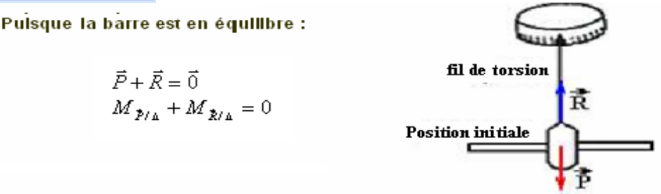
\includegraphics[width=0.5\textwidth]{./img/torsion_01.png}
\end{center}


\textbf{ Le deuxième équilibre:} Pour maintenir la barre en équilibre lorsque le fil est tordu d'un angle $\theta$ on exerce sur lui un couple de forces .
\begin{center}
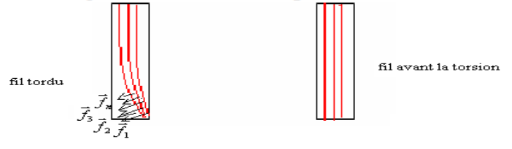
\includegraphics[width=0.4\textwidth]{./img/torion_00.png}
\end{center}
\begin{center}
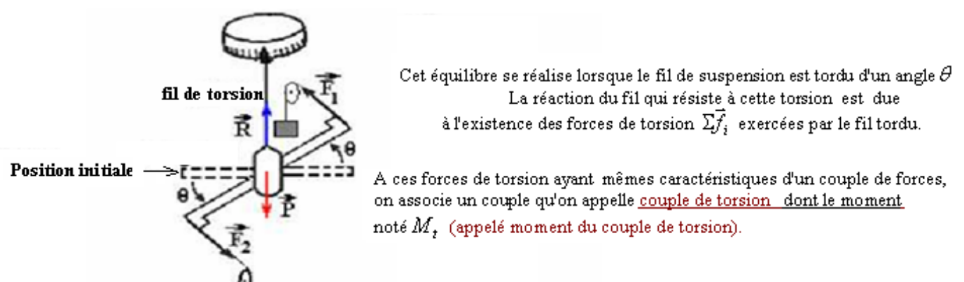
\includegraphics[width=1\textwidth]{./img/torsion_03.png}
\end{center}


\textbf{Etude du 2ème équilibre:}
\begin{itemize}
	\item Système étudié :{la barre}

	\item Bilan des forces: les forces qui s'exercent sur la barre à l'équilibre sont :
		\begin{itemize}

			\item $\vec{R}$ : action du fil.
			\item $\vec{P}$ : poids de la barre.
			\item $\vec{F_1}$ et $ \vec{F_2}$ : Le couple de force dont le moment $M_c = F.d$
			\item Les forces de torsion $\sum{\vec{f_i}}$ dont le moment du couple de torsion $M_t$
		\end{itemize}
	\item la barre est en équilibre, donc $\sum{M_{\vec{F}/{\Delta}} = 0}$ et $\sum{\vec{F} = \vec{0}}$

	\item $\sum{\vec{F} = \vec{0}}$ donc $$\vec{R} + \vec{P}+\vec{F_1}+\vec{F_2} + \vec{\sum{f_i}} = \vec{0}  $$ 
		d'après le premier équilibre  On a :  $\vec{R} + \vec{P} = \vec{0}$

		aussi $\vec{F_1}+\vec{F_2} = \vec{0} $ d'après les caractéristique d'un couple de forces donc $\sum{\vec{f}} = \vec{0}$


	\item $\sum{M_{\vec{F}/{\Delta}} = 0}$ donc 
		$$M_{\vec{P}/{\Delta}}  + M_{\vec{R}/{\Delta}} + M_{\vec{C}/{\Delta}} +  M_{\vec{T}/{\Delta}}= 0$$ 

		avec $M_{\vec{R}/{\Delta}} = M_{\vec{R}/{\Delta}} = 0$
		alors $$M_{\vec{C}/{\Delta}} =  -M_{\vec{T}/{\Delta}}$$
\end{itemize}


\subsection{Etude expérimentale: }

On fait varier le moment du couple de forces exercée sur la barre en modifiant l'intensité de la force commune F ou bien la
distance d entre les droites d'action des deux forces et on mesure la valeur de l'angle de torsion $\theta$.


\begin{center}
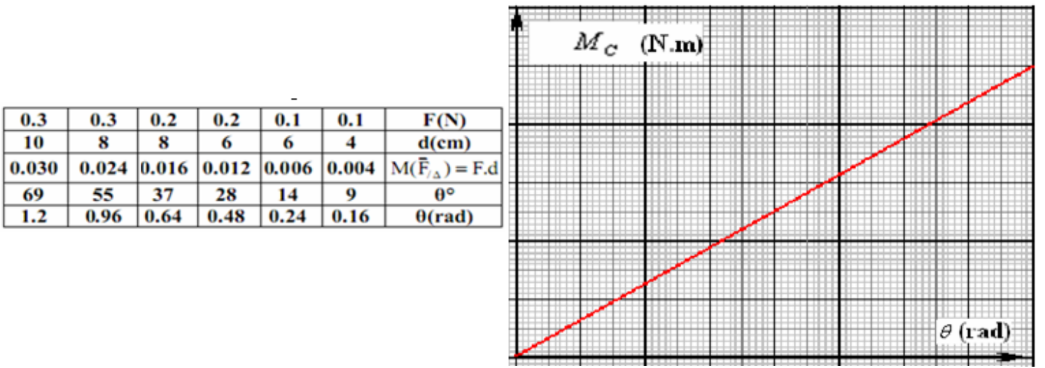
\includegraphics[width=1\textwidth]{./img/tor00.png}
\end{center}




Quand le solide tourne autour de l'axe du fil, celui-ci réagit à la torsion en exerçant des forces de rappel équivalentes à un couple dont le moment par rapport à l'axe est proportionnel à l'angle de torsion $\theta$en (rad) :
$$
\mathscr{M}_\Delta =-C.\theta
$$
\begin{center}
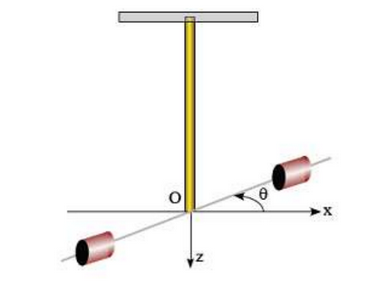
\includegraphics[width=0.4\textwidth]{./img/img_04.png}\\
\end{center}
La constante C dite constante de torsion dépend de la longueur et du diamètre du fil (supposé cylindrique) et
de la nature du matériau constituant le fil en N.m/rad.












\end{document}
